\section{Cel}
Celami tej części projektu były:
\begin{itemize}
    \item zaplanowanie fizycznej budowy,
    \item zaprojektowanie układu elektronicznego,
    \item wybranie i pozyskanie odpowiednich części,
    \item fizyczne skonstruowanie maszyny.
\end{itemize}

\section{Korpus}
Robot z założenia miał poruszać się na kołach, więc nieodzowne były silniki i podwozie.
Ze względu na brak doświadczenia w konstrukcji pojazdów, zdecydowano się na dobranie gotowego rozwiązania.
Na rynku znaleziono produkt będący zestawem do budowy robota jeżdżącego.
Składa się on z:
\begin{itemize}
    \item dwóch podstaw o rozmiarze 26 x 15 cm,
    \item czterech silników prądu stałego z przekładnią zasilanych napięciem 6V, o momencie obrotowym 0,78 Nm i poborze prądu 0,19 - 1,0 A,
    \item czterech kół z gumowymi oponami o średnicy 6,5 cm,
    \item elementów montażowych -- śrubki, dystanse, nakrętki itp.
\end{itemize}
Zawartość zestawu przedstawiona jest na zdjęciu \ref{rys:podwozie}.
\begin{figure}[!hb]
    \centering 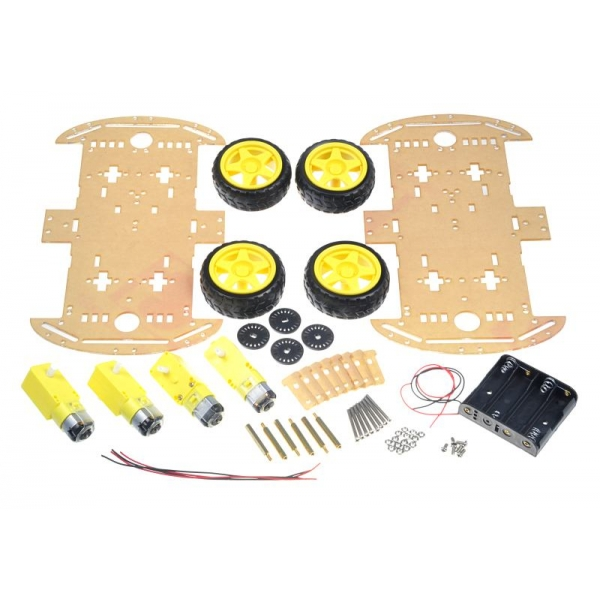
\includegraphics[width=0.618\linewidth]{podwozie.jpg}
    \caption{Gotowa platforma do budowy robota jeżdżącego}
    \label{rys:podwozie}
\end{figure}

Zdecydowano, że biorąc pod uwagę masę konstrukcji, cztery koła jezdne nie są potrzebne i dwa przednie powinny wystarczyć.
Na tył robota przeznaczono obrotowe kółko podporowe.
Dzięki takiemu rozwiązaniu zostaje więcej miejsca na umiejscowienie innych komponentów pomiędzy platformami.
Liczne otwory montażowe w podwoziu zostały wykorzystane do umocowania różnych elementów maszyny.

\section{Elektronika}
Wymagania stawiane względem oprogramowania robota były dosyć wysokie -- strumieniowanie obrazu z kamery, serwowanie aplikacji internetowej, gromadzenie danych.
Jednocześnie potrzebny był interfejs do sterowania silnikami, czy zbierania danych z czujników.
Platformą, która łączy świat pełnoprawnych komputerów i elektroniki jest popularne Raspberry Pi.
Konkretnym modelem wybranym do realizacji tego projektu jest Raspberry Pi 3B+.
Najważniejsze elementy specyfikacji:
\begin{itemize}
    \item wymiary 85 x 56 mm,
    \item 64-bitowy procesor ARM o taktowaniu 1.4GHz oraz 1GB RAM,
    \item karta graficzna Cortex-A53,
    \item karty Wi-Fi i Ethernet,
    \item cztery porty USB 2.0,
    \item porty: 4 x USB, HDMI, RCA, DSI (do wyświetlacza), CSI (do kamery), MicroSD,
    \item 40 pinów GPIO,
    \item napięcie zasilania 5V.
\end{itemize}

Pewną bolączkę stanowił dobór układu zasilania.
W porównaniu do np. Arduino, wadą Raspberry Pi jest mała tolerancja zakresu napięcia zasilania -- +- 5\%.
Ponadto nie posiada układów chroniących przed przepięciami, więc nie jest trudno spalić to urządzenie projektując nieodpowiedni układ lub zwyczajnie będąc nieostrożnym.
Wybrane do projektu silniki elektryczne wymagają wyższego napięcia - 6V.
Dodatkowym utrudnieniem jest charakterystyka silników prądu stałego, które generują zakłócenia na linii zasilania i mają wysoki prąd rozruchowy.

\label{motor_hat}
Z powyższych względów postawiono na gotowy układ projektowany pod Raspberry Pi.
Jest to nakładka \href{https://shop.sb-components.co.uk/products/motor-driver-hat-for-raspberry-pi}{\textit{Motor Driver Hat SKU21789}} od firmy SB Components, która zawiera:
\begin{itemize}
    \item dwukanałowy sterownik silników DC o napięciu 6 - 12 V o poborze prądu do 3A,
    \item generator sygnału PWM o rozdzielczości 12 bitów,
    \item regulator napięcia 5V do zasilania Raspberry Pi,
    \item interfejs komunikacyjny I2C.
\end{itemize}
Komponent ten, zamontowany na Raspberry Pi, przedstawiony jest na zdjęciu \ref{rys:motor_hat}.
\begin{figure}[!hb]
    \centering 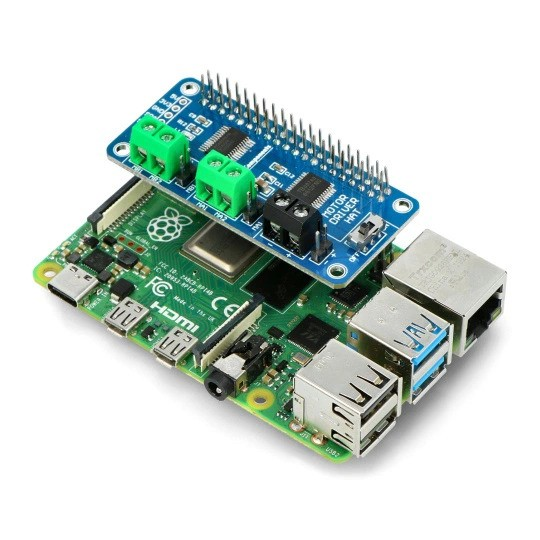
\includegraphics[width=0.618\linewidth]{motor_hat.jpg}
    \caption{Nakładka \textit{Motor Driver Hat SKU21789} na Raspberry Pi}
    \label{rys:motor_hat}
\end{figure}

\section{Zasilanie}
Ze względu na mobilność robota wybrano zasilanie akumulatorowe.
Dzięki zastosowaniu wyżej opisanego układu \ref{motor_hat}, zarówno płytkę Raspberry Pi z peryferiami, jak i silniki można zasilić z tego samego źródła.
Początkowo próbowano zastosować zwykłe baterie AA 1,5V, połączone szeregowo w celu uzyskania źródła napięcia 6V.
To rozwiązanie okazało się nieefektywne -- Raspberry Pi nawet nie było w stanie w całości przejść sekwencji bootowania.
Prawdopodobnie wykorzystane baterie AA nie mały wystarczającej wydajności prądowej.

Ostatecznie zastosowano dwie baterie litowo-jonowe 3,7V typu 18650 o pojemności 3,2 Ah połączone szeregowo.
Mają one wydajność prądową klasy 2C, co oznacza, że można z nich pobierać nawet 6,4 A prądu.
Rozwiązanie to sprostało wyzwaniu jednoczesnego zasilenia mikrokomputera z peryferiami i silników.
Dodatkową stabilność zapewniło podłączenie równolegle dwóch kondensatorów elektrolitycznych o łącznej pojemności 4800 $\mu$F w celu złagodzenia chwilowych spadków napięcia.

\section{Schemat układu}
Połączenie części elektronicznych jest przedstawione na schemacie \ref{rys:schemat}.
\begin{figure}[!hb]
    \centering 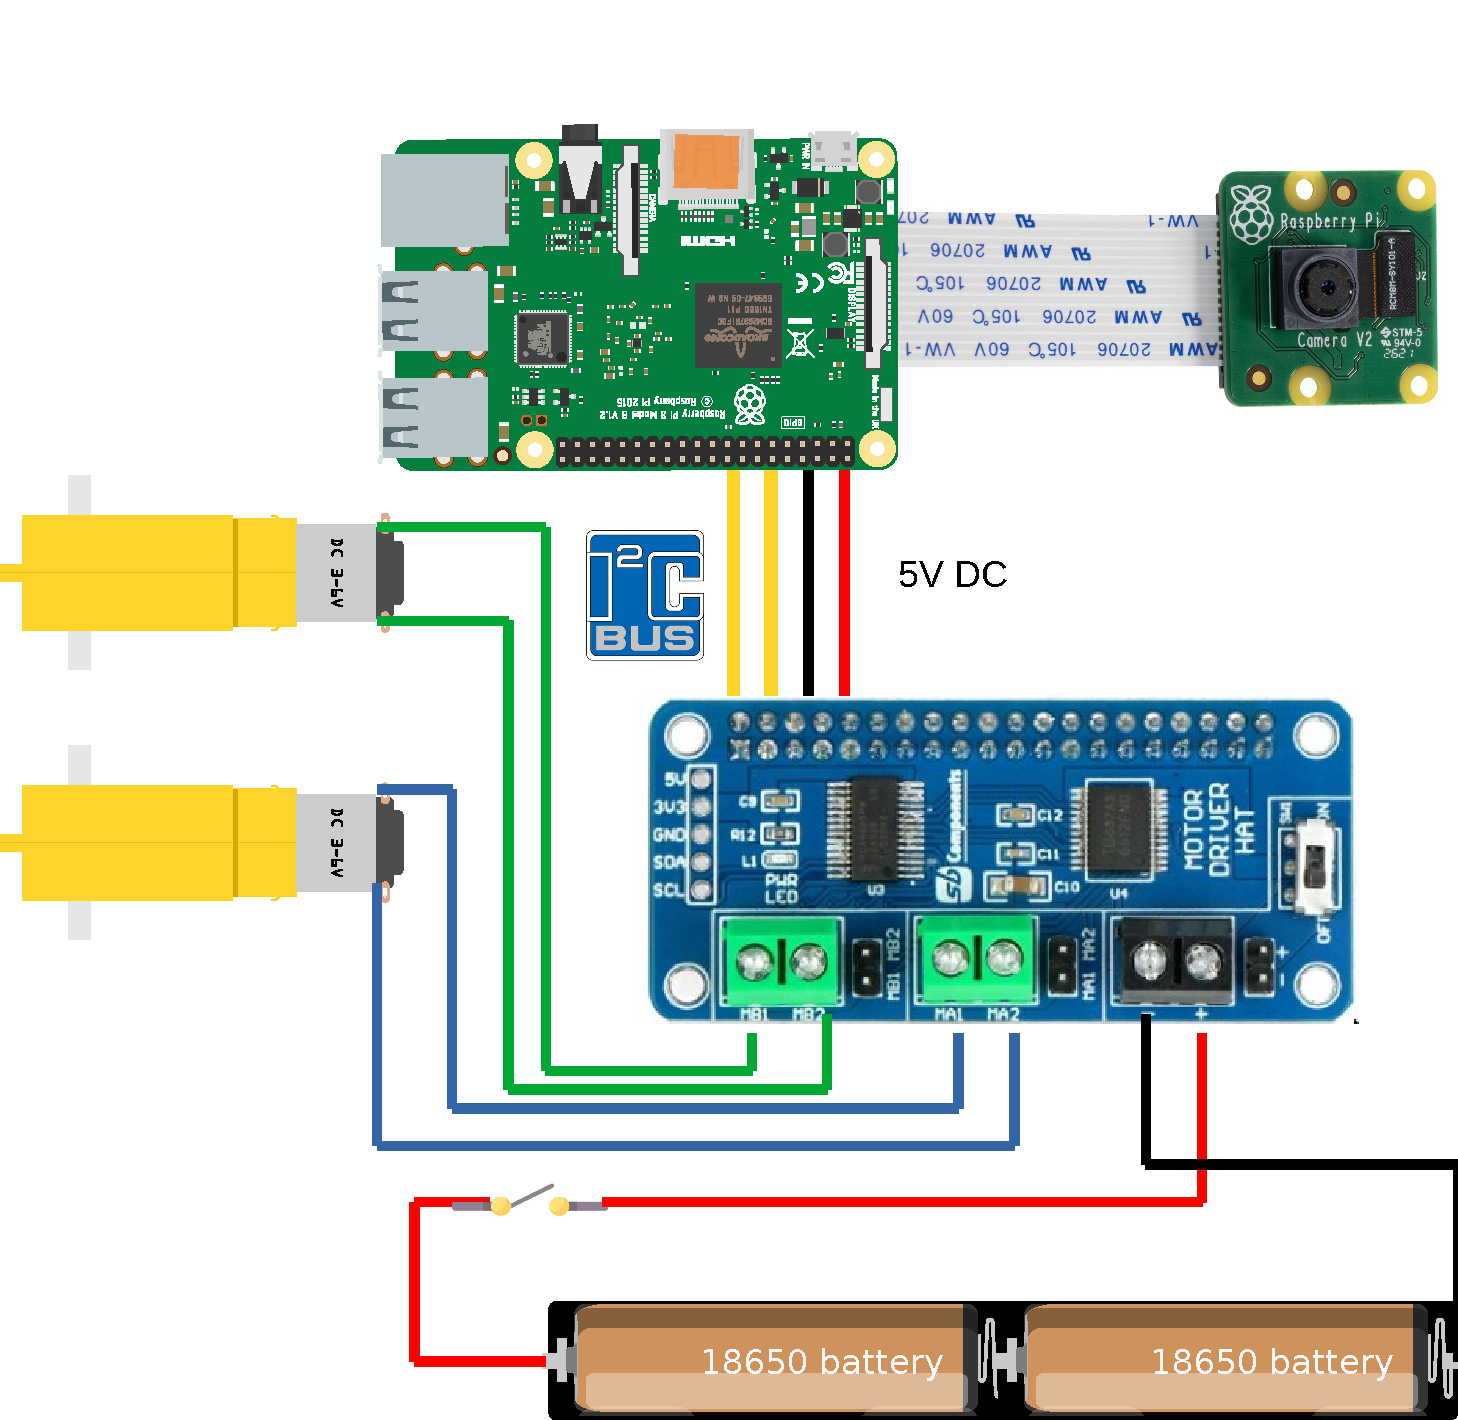
\includegraphics[width=1.0\linewidth]{schemat.pdf}
    \caption{Schemat połączeniowy}
    \label{rys:schemat}
\end{figure}

\section{Złożona konstrukcja}
Po złożeniu podwozia i zamontowaniu połączonych elementów elektronicznych konstrukcja była ukończona.
Efekt końcowy przedstawiają zdjęcia robota z góry \ref{rys:robot_top}, z przodu \ref{rys:robot_front}, z prawego boku \ref{rys:robot_right}, z lewego boku \ref{rys:robot_left} i z tyłu \ref{rys:robot_back}.
\begin{figure}[!hb]
    \centering 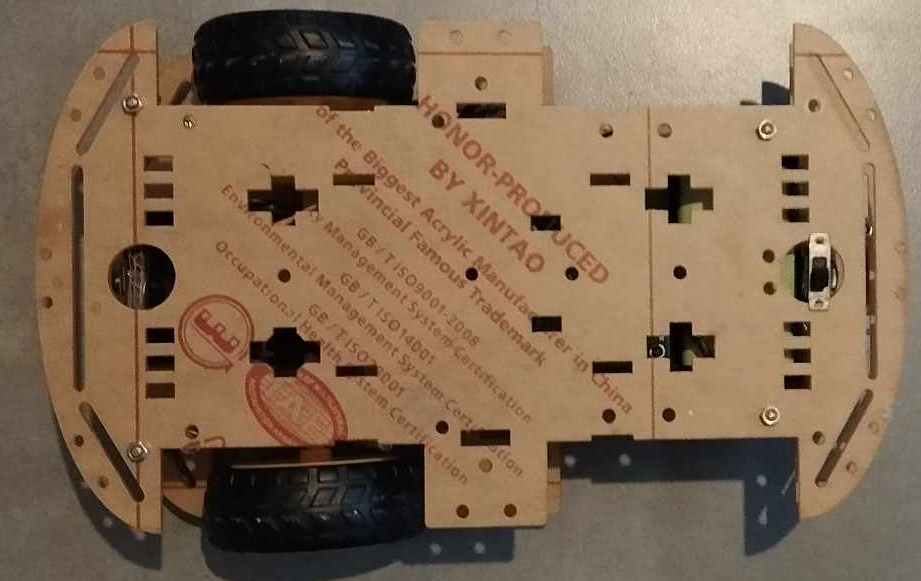
\includegraphics[width=0.618\linewidth]{robot_top.png}
    \caption{Zdjęcie robota z góry}
    \label{rys:robot_top}
\end{figure}
\begin{figure}[!hb]
    \centering 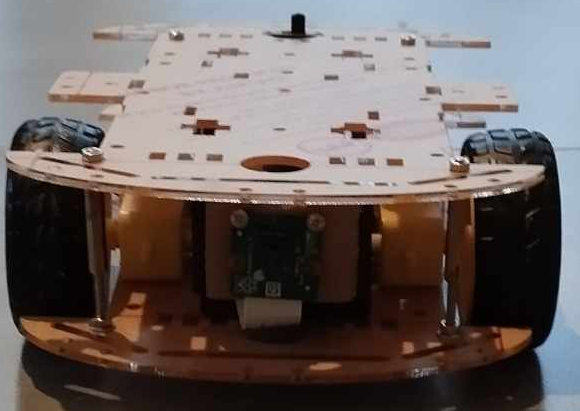
\includegraphics[width=0.618\linewidth]{robot_front.png}
    \caption{Zdjęcie robota z przodu}
    \label{rys:robot_front}
\end{figure}
\begin{figure}[!hb]
    \centering 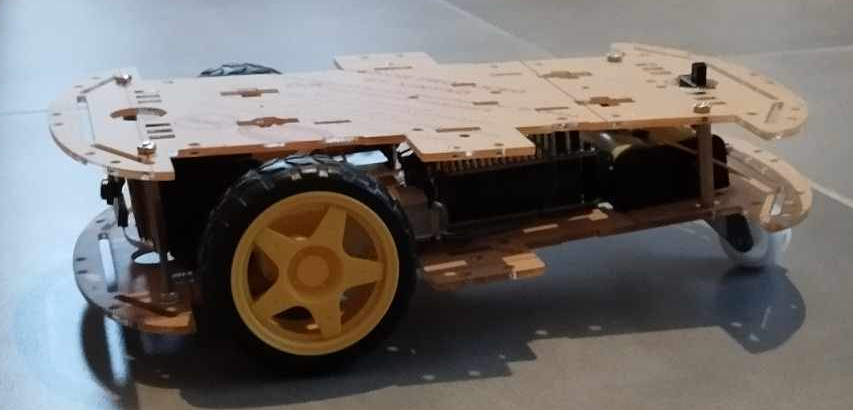
\includegraphics[width=0.618\linewidth]{robot_right.png}
    \caption{Zdjęcie robota z lewej strony}
    \label{rys:robot_left}
\end{figure}
\begin{figure}[!hb]
    \centering 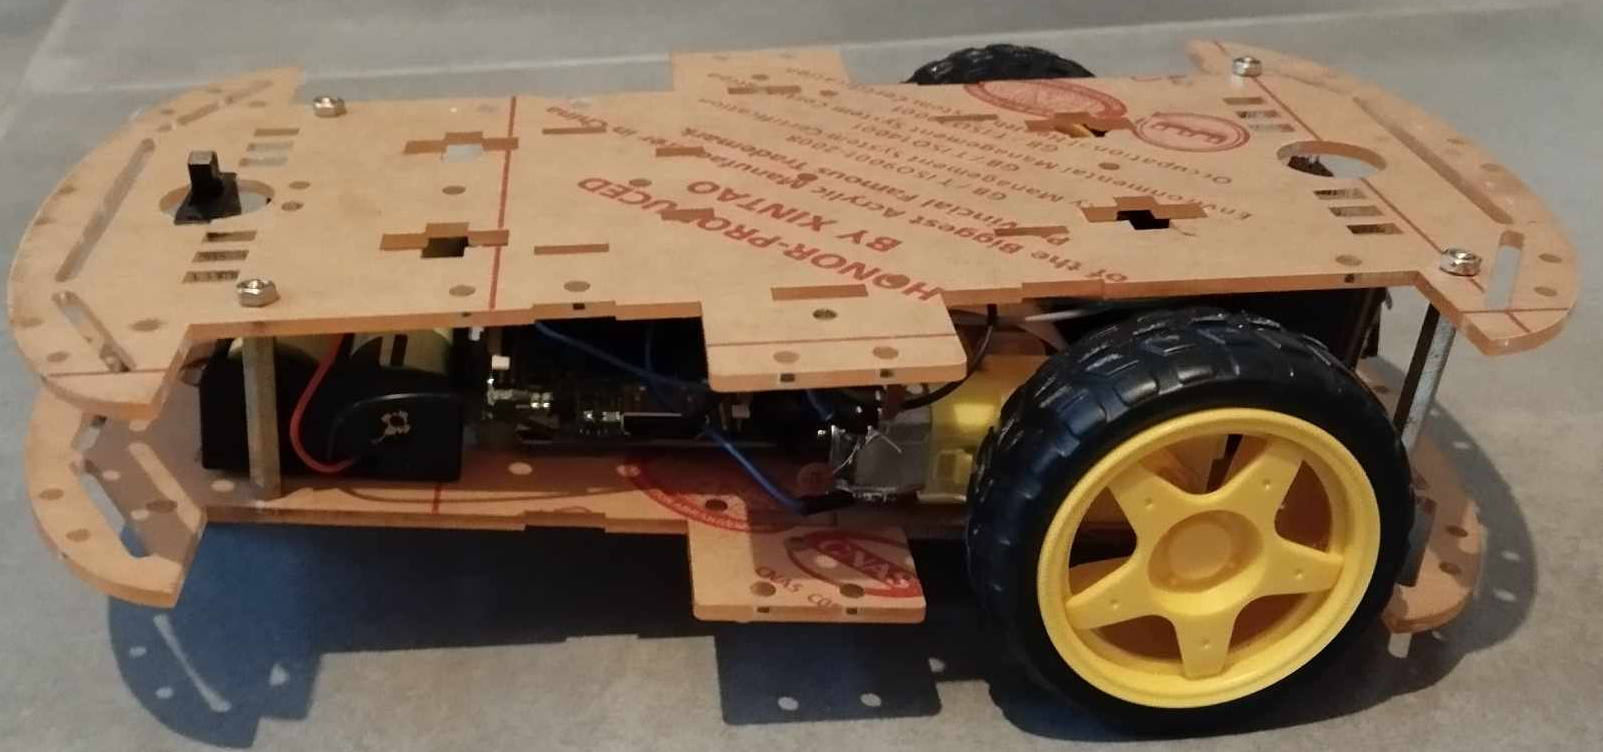
\includegraphics[width=0.618\linewidth]{robot_left.png}
    \caption{Zdjęcie robota z prawej strony}
    \label{rys:robot_right}
\end{figure}
\begin{figure}[!hb]
    \centering 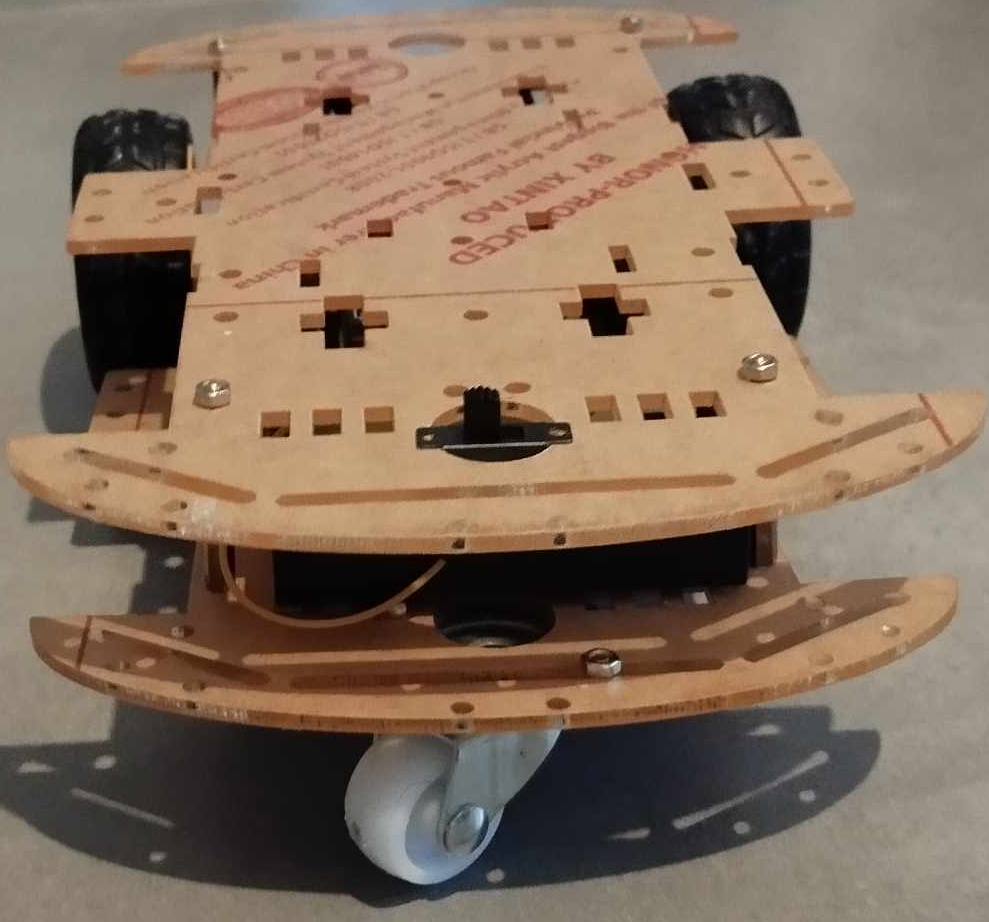
\includegraphics[width=0.618\linewidth]{robot_back.png}
    \caption{Zdjęcie robota z tyłu}
    \label{rys:robot_back}
\end{figure}
